
\documentclass[aspectratio=169, handout]{beamer}

%\usepackage[table]{xcolor}
\mode<presentation> {
\setbeamercovered{transparent}
  \usetheme{Boadilla}

%  \usetheme{Pittsburgh}
%\usefonttheme[2]{sans}
\renewcommand{\familydefault}{cmss}
%\usepackage{lmodern}
%\usepackage[T1]{fontenc}
%\usepackage{palatino}
%\usepackage{cmbright}
 
\useinnertheme{rectangles}
}
\usepackage{amsmath}
\setbeamercolor{normal text}{fg=black}
\setbeamercolor{structure}{fg= blue}
\definecolor{trial}{cmyk}{1,0,0, 0}
\definecolor{trial2}{cmyk}{0.00,0,1, 0}
\definecolor{darkgreen}{rgb}{0,.4, 0.1}
\usepackage{array}
\beamertemplatesolidbackgroundcolor{white}  \setbeamercolor{alerted
text}{fg=red}
\usepackage{tcolorbox}
\setbeamertemplate{caption}[numbered]\newcounter{mylastframe}

\font\domino=domino
\def\die#1{{\domino#1}}
\usepackage{tikz}
\usetikzlibrary{arrows}
\usepackage{colortbl}

\renewcommand{\familydefault}{cmss}
%\usepackage[all]{xy}

\usepackage{tikz}
\usepackage{lipsum}

 \newenvironment{changemargin}[3]{%
 \begin{list}{}{%
 \setlength{\topsep}{0pt}%
 \setlength{\leftmargin}{#1}%
 \setlength{\rightmargin}{#2}%
 \setlength{\topmargin}{#3}%
 \setlength{\listparindent}{\parindent}%
 \setlength{\itemindent}{\parindent}%
 \setlength{\parsep}{\parskip}%
 }%
\item[]}{\end{list}}
\usetikzlibrary{arrows}

\usecolortheme{lily}

\newtheorem{com}{Comment}
\newtheorem{lem} {Lemma}
\newtheorem{prop}{Proposition}
\newtheorem{condition}{Condition}
\newtheorem{thm}{Theorem}
\newtheorem{defn}{Definition}
\newtheorem{cor}{Corollary}
\newtheorem{obs}{Observation}
 \numberwithin{equation}{section}
 
\makeatletter
\def\beamerorig@set@color{%
  \pdfliteral{\current@color}%
  \aftergroup\reset@color
}
\def\beamerorig@reset@color{\pdfliteral{\current@color}}
\makeatother
\setbeamertemplate{navigation symbols}{}

\useoutertheme{miniframes}
\title[PLSC 30700]{Linear Models Lecture 1}

\author{Robert Gulotty}
\institute[Chicago]{University of Chicago}
\vspace{0.3in}


\begin{document}


\begin{frame}
\maketitle
\end{frame}



\begin{frame}
\frametitle{Goals}
\begin{itemize}
\item We will be modeling data.
\begin{itemize}
\item Summarizing complex data with less complicated formula (data reduction).
\item Drawing inferences about causal processes.
\item Making predictions.
\end{itemize}
\item To do so, we will either
\begin{itemize}
\item Make direct assumptions about the way the data was generated.
\item Use statistical theory to approximate the way the data was generated.
\end{itemize}
\item  In both cases, we use random variables called `statistics', their distributions and their relations.
\item Today we review the mathematics of random variables, their distributions, and their summaries.
\end{itemize}
\end{frame}


\section{Probability Rules}
\begin{frame}
\frametitle{Basic Ideas of Probability}

Probability models random phenomenon with three ingredients:\pause 
\begin{itemize}
\item[1)] \textbf{Sample space}: \{all possible outcomes of a random process\} \pause 
\item[2)] \textbf{Events}: \{subsets of all possible outcomes of a random process\} \pause 
\item[3)] \textbf{Probability Law}: a function $P(\cdot)$ which gives the relative chance of an event, a non-negative number.
\end{itemize}
\end{frame}

\begin{frame}{Founder of Axiomatic Probability}
\begin{center}
\includegraphics[width=1.5 in]{images/Kolmogorov.jpeg}\\
Kolmogorov (1933).
\end{center}
\end{frame}

\begin{frame}
\frametitle{Sample Spaces: All Things that Can Happen}

\begin{defn}
The \alert{sample space} is the set of all things that can occur.  This set is often referred to by the symbol $\Omega$ or $S$.
\end{defn}
\pause 
{Examples: } \pause 
\begin{itemize}
\item[1)] Discrete: The outcome of two dice 
\begin{itemize}
\item[-] $\Omega = \{$\die1\die1, \die1\die2 ,  $\hdots,$ \die6\die6$ \}$ \pause
\end{itemize}
\item[2)] Continuous: Value of a house
\begin{itemize}
\item[-] $\Omega = \{t: t\in \mathbb{R}\}$ 
\end{itemize}\pause 
\item[3)] Continuous: Survival of Monarch 
\begin{itemize}
\item[-] $\Omega = \{t: 0\leq t \leq 120\}$ 
\end{itemize}

\end{itemize}
\end{frame}


\begin{frame}
\frametitle{Probability Law}
\begin{itemize}
\item \alert{Probability}: chance of event.
\begin{itemize}
\item[-] A function $P: \Omega \rightarrow [0,1]$
\item[-] Describes relative likelihood of events.
\end{itemize}\pause 
\item Given an event $A$, $P(A)$ quantifies the chance it occurs.\pause 
\item Let $E=\{x : x \in(a,\ b)\}$ be an event.
$$P(E)=\int_{x \in E} f_X(x) dx$$
\item[] where $f_X(x)$ is the *probability density function*, e.g.
\begin{itemize}
\item Normal distribution: dnorm(x, $\mu$, sd)
\item t distribution: dt(x, df)
\item F distribution: df(x, df1, df2)
\end{itemize}
\item Note: the probability of continuous events are only positive for \emph{intervals}.
\end{itemize}
\end{frame}


\begin{frame}
\frametitle{Example: Candidate heights}
\begin{itemize}
\item What is the probability a male candidate would be at least 72 inches tall by chance?
$$\Omega = \{h: 20 \leq h \leq 108\}, \quad E = \{h: 72 \leq h \leq 108\}$$\pause 
\item Male heights are close to a normal distribution with mean ($\mu$) 70 inches with a standard deviation ($\sigma$) of 3 inches.
$$f_H(h) =dnorm(h, \mu= 70, sd = 3)$$
\begin{align*}
P(E)&=\int_{72}^{108} f_H(h) dh\\\pause
&= integrate(dnorm, lower=72, upper=108, mean= 70, sd = 3)
&=.252
\end{align*}
\end{itemize}
\end{frame}



\begin{frame}
\frametitle{Aside on Calculating integrals}
\begin{itemize}
\item In R there is a function pnorm(x) that calculates the integral of the normal distribution from $-\infty$ to $x$.\pause 
\item We can then rewrite our problem in terms of these functions.
\begin{align*}
P(E)&=\int_{72}^{108} f_H(h) dh\\\pause
&=\int_{-\infty}^{108} f_H(h) dh-\int_{-\infty}^{72} f_H(h) dh\\\pause
&= F(H \leq 108)-F(H \leq 72) \ \quad \quad \textit{where F() is the anti-derivative of f()}\\\pause
&=pnorm(108, 70, 3) - pnorm(72, 70, 3)\\\pause
&=1-0.747
\end{align*}
\end{itemize}
\end{frame}


\begin{frame}
\frametitle{Example: Short and Tall}
\begin{itemize}
\item What is the probability a male candidate would either at least 72 inches tall or below 65 inches?
\begin{align*}
E_1 &= \{h: 72 \leq h \leq 108\}\\
E_2 &= \{h: 20 \leq h \leq 65\}\\\pause
E&= E_1\cup E_2\\\pause
P(E)&= P(E_1\cup E_2)=P(E_1)+P(E_2)-P(E_1\cap E_2)\\\pause 
P(E_1\cup E_2)&=\int_{20}^{65} f_H(h) dh+\int_{72}^{108} f_H(h) dh-0\\\pause
&= [F(H \leq 65)-F(H \leq 20)]+0.25\\\pause
&=[pnorm(65, 70, 3)-0] +0.25\\\pause
&=.048+0.25
\end{align*}
\end{itemize}
\end{frame}

\begin{frame}{Formalizer of Bayes' Rule}
\begin{center}
\includegraphics[width=1.8 in]{images/Richard_Price_West.jpeg}\\
Price (1784).
\end{center}
\end{frame}




\begin{frame}
\frametitle{Definition of Conditional Probability}
The \emph{conditional probability} of an event A given an event B is given by:
$$P(A|B)=\frac{P(A\cap B)}{P(B)}\quad \text{for all }P(B)\neq 0$$
\\
$P(A\cap B)$ is called the joint probability.\\
\pause We can rearrange this to form the``Multiplication Rule'':
$$P(A\cap B)=P(A|B)P(B)$$

\end{frame}


\begin{frame}
\frametitle{Examples of Conditional probability}
If A is Trump runs again, and B is the event that Trump wins:
$$P(A|B)=\frac{P(A\cap B)}{P(B)}=\frac{P(B)}{P(B)}=1$$\pause
$$P(B|A^c)=\frac{P(B\cap A^c)}{P(A^c)}=\frac{0}{P(A^c)}=0$$

\end{frame}



\begin{frame}
\frametitle{Law of Total Probability}

\begin{itemize}
\item $E_1,\  E_2$ are mutually exclusive if $E_1\cap E_2=\emptyset$

\item If a given set of mutually exclusive events, $E_1,\  E_2,\ E_3\ldots E_n$, their union forms the sample space $\Omega$ we say $E_1,\  E_2,\ E_3 \ldots E_n$ \emph{partitions} the sample space. \\ 
\begin{center}
\includegraphics[width=2.5 in]{images/law-total-probability-diagram.png}
\end{center}
\item Divide and conquer: turn big problem into small problems:
\begin{thm}
Law of Total Probability: 
Given such a partition, the probability of any event A is:

$$P(A)= P(A|E_1)P(E_1)+P(A|E_2)P(E_2)+...+P(A|E_n)P(E_n)$$
\end{thm}
\end{itemize}

\end{frame}


\begin{frame}
\frametitle{Proof of Law of Total Probability}
\begin{proof} 
\begin{align*}
P(A) &= P(A\cap \Omega) && \text{because }A\subseteq \Omega \\\pause
P(A) &= P(A\cap (E_1\cup E_2 \cup ... \cup E_n))  && \text{E partitions }\Omega \\\pause
P(A) &= P((A\cap E_1)\cup (A\cap E_2) \cup ... \cup(A\cap E_n))  && \text{Distributive Law}\\ \pause
P(A) &=  P(A\cap E_1)+ P(A\cap E_2) + ...P(A\cap E_n)&& E_i\cap E_j=\emptyset\\\pause
P(A) &=  P(A|E_1)P(E_1)+P(A|E_2)P(E_2)+...+P(A|E_n)P(E_n)&&\text{multiplication rule}
\end{align*}

\end{proof}

\end{frame}



\begin{frame}{Independence}

\begin{defn}
Suppose we have two events $E_{1}, E_{2}$.  We say these events are \alert{independent} if:
\begin{align*}
P(E_{1}\cap E_{2}) &= P(E_{1}) P( E_{2})
\end{align*}
\end{defn}
\begin{itemize}
\item To discover the systematic component of the experiment, we need to make assumptions about what affects what.\pause
\item The most important assumption is the notion of independence.
\end{itemize}
\end{frame}



\begin{frame}
\frametitle{Independence and Information} 

Does one event provide \alert{information} about another event? \pause 

\begin{defn} 
If B does not change the probability that A occurs, A is independent of B.
\begin{align*}
P(A|B)&=P(A)\\ \pause
 P(A|B)&=\frac{P(A\cap B)}{P(B)}=\frac{P(A)P(B)}{P(B)}=P(A)
 \end{align*}
\end{defn}
\pause

Independence is symmetric: if $F$ is independent of $E$, then
  $E$ is independent of $F$

\end{frame}


\begin{frame}
\frametitle{Conditional Independence}

\begin{defn}
Let $E_{1}$ and $E_{2}$ be two events.  We will say that the events are conditionally independent given $E_{3}$ if 
\begin{align*}
P(E_{1} \cap E_{2} | E_{3}) &= P(E_{1} | E_{3} ) P(E_{2} | E_{3} ) 
\end{align*}
\end{defn}

\end{frame}

\begin{frame}
\frametitle{Amusement Park Example}
\begin{columns}
\begin{column}{0.7\textwidth}
\begin{itemize}
\item There is a strong correlation between child height and literacy (a spurious relationship).
\item Suppose there is an Amusement Park popular with 1st graders (6-7 year olds).
\item Can we rely on the children understanding this sign?
\end{itemize}
\end{column}
\begin{column}{0.3\textwidth}
\includegraphics[width=2 in]{images/carnival.jpeg}
\end{column}
\end{columns}
\end{frame}

\begin{frame}
\frametitle{Statistical Model of Height and Literacy}
\begin{itemize}
\item $x$ is the height of a child where $f(x)=N(\mu=33+z*2, s= 1.2)$.\
\item $y$ is \# words the child knows $f(y)=N(\mu=100+z*150, s= 200)$.\pause 
\item $z$ is the child's age, where $f(z)=\begin{cases} 6\text{ with probability }1/2\\ 7\text{ with probability }1/2\end{cases}$
\item The probability that a first grader can read the "you must be this tall sign" and is at least 48'' tall:
$$P(A\cap B)\text{ where }A=\{x: x>48\}, \ B=\{y: y>1400\}$$
\end{itemize}
\end{frame}

\begin{frame}
\begin{center}
\includegraphics[width=5 in]{images/Heightdensity.png}
\end{center}
\end{frame}

\begin{frame}
\begin{center}
\includegraphics[width=5 in]{images/Wordsdensity.png}
\end{center}
\end{frame}

\begin{frame}{Using Law of Total Probability}
\begin{align*}
A&=\{x: x>48\}\\\pause 
P(A)&=P(A|Z=6)*P(Z=6)+P(A|Z=7)*P(Z=7) \tag{Law of Total Probability}\\\pause 
&=[\int_{48}^\infty \phi(x|45,1.2)dx]*P(Z=6)+[\int_{48}^\infty \phi(x|47,1.2)dx]*P(Z=7)\\\pause 
&=(1-pnorm(48, 45, 1.2) )*1/2+(1-pnorm(48, 47, 1.2) )*1/2\\\pause 
&=0.104\\\pause 
\end{align*}
By similar reasoning, $B=\{y: y>1400\}$, $P(B)=.06$.\\
\end{frame}




\begin{frame}{Using conditional independence}
We know $height$ and $literacy$ are conditionally independent.
\begin{align*}
P(A\cap B)&=P(A\cap B|Z=6)P(Z=6)+P(A\cap B|Z=7)P(Z=7)\\ \pause
&=P(A|Z=6)P(B|Z=6)P(Z=6)+P(A|Z=7)P(B|Z=7)P(Z=7)\\\pause
&=(1-pnorm(48, 45,1.2) )*(1-pnorm(1400, 1000, 200) )*1/2+\\
&\quad (1-pnorm(48, 47, 1.2) )*(1-pnorm(1400, 1150, 200) )*1/2 \\\pause
&=.01
\end{align*}
\end{frame}

\begin{frame}
\begin{center}
\includegraphics[width=5 in]{images/Heightwords.png}
\end{center}
\end{frame}

\begin{frame}
\begin{center}
\includegraphics[width=5 in]{images/Heightwordsage.png}
\end{center}
\end{frame}

\begin{frame}

\begin{table}[!htbp] \centering
\begin{tabular}{@{\extracolsep{5pt}}lcc} 
\\[-1.8ex]\hline 
\hline \\[-1.8ex] 
 & \multicolumn{2}{c}{\textit{DV: height}} \\ 
\cline{2-3} 
\\[-1.8ex] & (1) & (2)\\ 
\hline \\[-1.8ex] 
 words & 0.002$^{***}$ & 0.0002 \\ 
  & (0.001) & (0.0004) \\ 
  & & \\ 
 ages &  & 1.976$^{***}$ \\ 
  &  & (0.183) \\ 
  & & \\ 
 Constant & 44$^{***}$ & 32.8$^{***}$ \\ 
  & (0.552) & (1.130) \\ 
  & & \\ 
\hline \\[-1.8ex] 
Observations & 200 & 200 \\ 
R$^{2}$ & 0.057 & 0.407 \\ 
\hline 
\hline \\[-1.8ex] 
\end{tabular} 
\end{table} 

\end{frame}

\section{Random Variables}

\begin{frame}
\frametitle{Random Variables}
Given a sample space $\Omega$, and a probability law $P$:
\begin{defn}
A \emph{random variable} is a \alert{function} that assigns real numbers (usually) to events in a sample space $\Omega$.
\end{defn}
$$X(\omega): \Omega \to \mathbb{R}$$

\end{frame}


\begin{frame}
\frametitle{Connecting random variables to probability}
\begin{itemize}
\item X assigns some numbers to events.\pause
$$X(\omega): \Omega \to \mathbb{R}$$
\item Remember, probability assigns a chance to an event.\pause
$$P(\omega): \Omega \to \mathbb{R}$$
\item What are the probabilities associated with $X(\omega)$?\pause
\end{itemize}
\end{frame}





\begin{frame}
\frametitle{Cumulative Distribution Function: F(x)} 

Random variables are characterized by cumulative distribution functions.\pause

\begin{defn} 
Cumulative Distribution function.  For a continuous random variable $X$ define its cumulative distribution function $F(\cdot )$ as, 
\begin{align*} 
F(x) &=P(\omega: X(\omega)\leq x)= P(X \leq x) = \int_{-\infty} ^{x} f(t) dt 
\end{align*}
\end{defn}
\end{frame}

\begin{frame}{PDFs, CDFs, OLS}
\begin{center}
\includegraphics[width=1.8 in]{images/Gauss.jpeg}\\
Gauss (1809)
\end{center}
\end{frame}

\begin{frame}
\frametitle{Probability Density Function: f(x)}
\begin{defn}
If X is a continuous random variable, the probability density function of X is the function $f_X(x)$ that satisfies.
\begin{align*}
F_X(x)&=P(X\leq x)\\
&=P(X\in (-\infty,\ x))\\
&=\int_{-\infty}^{x} f_X(t)dt\ \ \ \ x\in \textbf{R}
\end{align*}
\end{defn}
\pause

\begin{center}
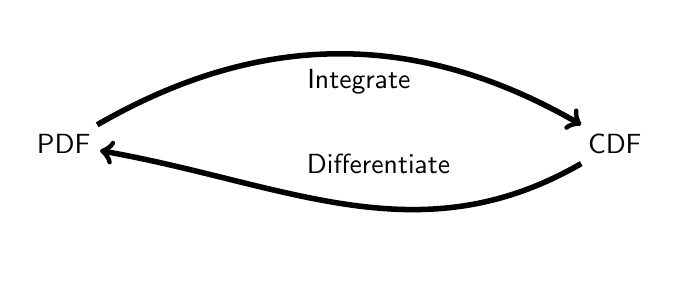
\begin{tikzpicture} 
\node (d1) at (-4, 3) [] {PDF};  
\node (f1) at (3, 3) [] {CDF} ; 
\draw[->, line width=2pt] (d1) to [out=30, in=150] (f1) ; 
\node (d2) at (-0.25, 3.8) [] {Integrate} ; 
\node (f2) at (0, 2.75) [] {Differentiate} ; 
\draw[->, line width=2pt] (f1) to [out=210, in=350] (d1) ; 
\end{tikzpicture}
\end{center}
\end{frame}



\begin{frame}
\frametitle{Example: continuous uniform}

\begin{defn}
Y has a uniform distribution on the interval $(a,b)$ if
$$f_Y(y)=\begin{cases} \frac{1}{b-a}& \text{if } a\leq y\leq b\\ 0 & \text{otherwise} \end{cases}$$
$$F_Y(y)=\begin{cases} 1 & \text{if } b<y\\\frac{y-a}{b-a}& \text{if } a<y<b\\ 0 & \text{if } y<a\ \end{cases}$$
\end{defn}

\end{frame}
\begin{frame}{Example: Uniform}

Example: Suppose that we are waiting for Comcast to show up and install our cable package.  They say that they may arrive between 2:00 and 8:00.  Without any further information, you may have no reason to suspect any particular time over any other.
$$X\sim U(2,8)$$

\end{frame}



\begin{frame}
\frametitle{Example: PDF of continuous uniform}
\begin{center}
\includegraphics[width=4 in]{images/Udists2.pdf}
\end{center}

\end{frame}




\begin{frame}
\frametitle{Example: continuous uniform }
What is the probability that the cable installation truck arrives before 4:00?

\end{frame}


\begin{frame}
\frametitle{Example: CDF of continuous uniform ($P(X\leq4)$)}
\begin{center}
\includegraphics[width=3.5in]{images/Udists3.pdf}
\end{center}

\end{frame}




\begin{frame}
\frametitle{Example: continuous uniform}

$$P(Y\leq y)=\int_{x=-\infty}^{y}f(x)dx=\int_{x=-\infty}^{y}\frac{1}{b-a}dx=\int_{x=a}^{y}\frac{1}{b-a}dx$$\pause
$$\frac{y}{b-a}-\frac{a}{b-a}=\frac{y-a}{b-a}$$\pause
 $$=\frac{4-2}{8-2}$$

\end{frame}



\begin{frame}
\frametitle{Example: continuous uniform}
\begin{center}
\includegraphics[width=3.5 in]{images/Udists4.pdf}
\end{center}

\end{frame}



\section{Expectation}

\begin{frame}
\frametitle{Definition of Expectation}

What can we \alert{expect} from a trial? \pause \\

The expectation is the \textbf{value} of random variable weighted by the \textbf{probability} of observing that outcome.\pause

\begin{defn} 
Expected Value: define the expected value of a function $X$ as, 
\begin{align*}
E[X] &=  \sum_{x:p(x)>0} x p(x) &&\text{when x is discrete} \\ 
E[X] &=  \int_{-\infty}^{\infty} x f(x) dx &&\text{when x is continuous}
\end{align*}
In words: for all values of $x$ with $p(x)$ greater than zero, take the sum/integral of values times weights.
\end{defn} 

\end{frame}




\begin{frame}{$E(X)= \sum_{x:p(x)>0} x *p(x) =0*.75+2*.25= \frac{1}{2}$}

\begin{center}
 \includegraphics[width=3.5 in]{images/plot1.png}
\end{center}

\end{frame}


\begin{frame}{$E(X)= \sum_{x:p(x)>0} x *p(x) =0*.6+2*.2+6*.2= 1.6$}

\begin{center}
\includegraphics[width=3.5 in]{images/plot2.png}
\end{center}

\end{frame}



\begin{frame}{$E(X)= \sum_{x:p(x)>0} x* p(x) =0*.6+2*.2+9*.2= 2.2$}

\begin{center}
\includegraphics[width=3.5 in]{images/plot3.png}
\end{center}

\end{frame}


\begin{frame}
\frametitle{Expectation Properties}
\begin{align*}
E[X+Y]&=E[X]+E[Y]\\
E[a]&=a\\
E[aX]&=aE[X]\\
E[E[X]]&=E[X]\\
E[XY]&\neq E[X]\times E[Y]
\end{align*}
\end{frame}


\begin{frame}
\frametitle{Properties of the Expectation}
$$E[a]=a$$\pause 
Proof:  Suppose Y is a random variable such that $Y = a$ with probability 1 and $Y= 0$ otherwise:
\begin{align*}
E[Y] &= \sum_{y: p(y)>0} y p(y) \pause\\
&= a p(Y=a)+ 0* p(Y=0) \pause\\
&= a*1  + 0  \\
&= a 
\end{align*}


\end{frame}


\begin{frame}{Justification of Expectation}
If we want to predict $y$ with no other information, and our prediction is called $\pi$, one standard for prediction is to minimize the mean-square error:
\begin{align*}
M &= \int (y -\pi)^2 f(y) dy\\\pause
&=E[(y-\pi)^2]\\\pause
&=E[y^2-2\pi y+\pi^2]\\\pause
&=E[y^2]-E[2\pi y]+E[\pi^2]\\\pause
&=E[y^2]-2\pi E[y]+ \pi^2\pause
\end{align*}
Using calculus to minimize:\pause
\begin{align*}
\frac{\partial M}{\partial \pi}&=-2E[y]+ 2\pi\\\pause
\pi&=E[y]
\end{align*}
\end{frame}



\begin{frame}
Suppose $X \sim Uniform(3,5)$.  What is $E[X]$? \pause 
\begin{align*}
E[X]  &= \int_{-\infty}^{\infty} xf(x)dx   \pause \\
&= \int_{-\infty}^{3} x 0 dx + \int_{3}^{5} x \frac{1}{5-3}dx + \int_{5}^{\infty} x 0 dx \pause  \\
&= 0 +  \frac{x^{2}}{4} |^{5}_{3} + 0   \pause \\
&= 0 + 5^2/4-3^2/4+ 0  \pause \\
&= 4 
\end{align*}


\end{frame}

\begin{frame}

\begin{cor} 
Suppose $X$ is a continuous random variable.  Then, 
\begin{align*}
E[aX + b] & =  aE[X] + b
\end{align*}
\end{cor}
\pause 

\begin{proof}
\begin{align*}
E[aX + b] & =  \int_{-\infty}^{\infty} (a x + b)f(x) dx \\ \pause 
& =  a \int_{-\infty}^{\infty} x f(x) dx + b \int_{-\infty}^{\infty} f(x)dx  \\ \pause 
& =  a E[X]  + b \times 1
\end{align*}


\end{proof}


\end{frame}





\section{Variance}

\begin{frame}
\frametitle{Second Moment: Variance} 

Expected value is a measure of \alert{central tendency}. \pause \\
What about spread? \pause  \alert{Variance}  \pause \\
\begin{itemize}
\item[-] For each value, we might measure distance from center \pause 
\begin{itemize}
\item[-] Distance, squared $d(x, E[x])^{2} = (x - E[x])^2$  \pause 
\end{itemize}
\item[-] Then we might take weighted average of these distances by taking an expectation. \pause 
\end{itemize}

\end{frame}

\begin{frame}{Two formulas for Variance}
\begin{align*} 
E[(X - E[X])^2] &= \sum_{x} (x  - E[X])^2p(x) \\  \pause 
& =  \sum_{x} \left(x^2  -E[X] x -x E[X] + E[X]^2\right) p(x)   \\  \pause 
& =  \sum_{x} \left(x^2  -2E[X] x  + E[X]^2\right) p(x)  \\  \pause 
& =  \sum_{x} x^2 p(x)   - \sum_{x} 2x E[X]p(x) + \sum_{x} E[X]^2 p(x)   \\  \pause 
& =  \sum_{x} x^2 p(x)   - 2E[X] \sum_{x} x p(x) + \sum_{x} E[X]^2 p(x)   \\  \pause 
& =  E[X^2] - 2E[X]^2 + E[X]^2  \\ \pause 
& =  E[X^2] - E[X]^2 =  \text{Var}(X)
\end{align*}
\end{frame}


\begin{frame}
\frametitle{Definition of Variance}

\begin{defn}
The variance of a random variable $X$, var$(X)$, is 
\begin{align*}
 \text{var}(X) &= E[(X - E[X])^2]  \\
 &=  \int_{-\infty}^{\infty} (x - E[X])^2f(x) dx \\
 &=   E[X^2] - E[X]^2 \
\end{align*}
\end{defn}

\begin{itemize}
\item[-] We will define the standard deviation of $X$, sd$(X) = \sqrt{\text{var}(X)} $
\item[-] var$(X) \geq 0$.  
\item[-] We use $\sigma^2$ to indicate variance.
\end{itemize}


\end{frame}


\begin{frame}
\frametitle{Variance Corollary} 

\begin{cor}
Var($aX  + b$)  = $a^2$Var($X$) 
\end{cor} 
\pause 

\textbf{Proof:} Define $Y = aX +b$.  We know that $Var(Y) = E[(Y - E[Y])^2]$. \pause 
\begin{align*}
& = E[ ((aX + b) - E[a X + b])^2 ]   \pause \\
& = E[ ((aX + b) - (a E[X] + b))^2 ]   \pause \\
& = E[ (aX -a E[X] )^2 ]  \pause \\
& =  E[ (a^2 X^2 - 2 a^2 X E[X] + a^2 E[X]^2)]  \pause \\
& =  a^2E[X^2] -2a^2E[X]^2 + a^2 E[X]^2   \pause \\
& =  a^2(E[X^2] - E[X]^2) \pause  \\
& =  a^2 Var(X) 
 \end{align*}
\end{frame}

\begin{frame}
\frametitle{Often the sample (co)variance appears in an alternative form:} 
\small{
\begin{align*}
\widehat{Var}(X)&=\frac{1}{N}\sum_i(x_i-\bar{x})(x_i-\bar{x})  \pause \\
& =\frac{1}{N}\sum_ix_i^2-\bar{x}x_i-x_i\bar{x}+\bar{x}\bar{x}  \pause \\
& =\frac{1}{N}\sum_ix_i^2-\bar{x}\frac{1}{N}\sum_ix_i-\bar{x}\frac{1}{N}\sum_ix_i+\frac{1}{N}\sum_i\bar{x}\bar{x}\\
& =\frac{1}{N}\sum_ix_i^2-\bar{x}\frac{1}{N}N\bar{x}-\bar{x}\frac{1}{N}\sum_ix_i+\bar{x}\bar{x} \tag{$\sum_i x_i=N\bar{x}$}\\
& =\frac{1}{N}\sum_ix_i^2-\bar{x}\frac{1}{N}\sum_ix_i \tag{$\bar{x}\bar{x}$ cancel}\\
& =\frac{1}{N}\sum_i(x_i-\bar{x})x_i\\
 \end{align*}}
\end{frame}


\begin{frame}
\begin{columns}
\begin{column}{0.5\textwidth}
  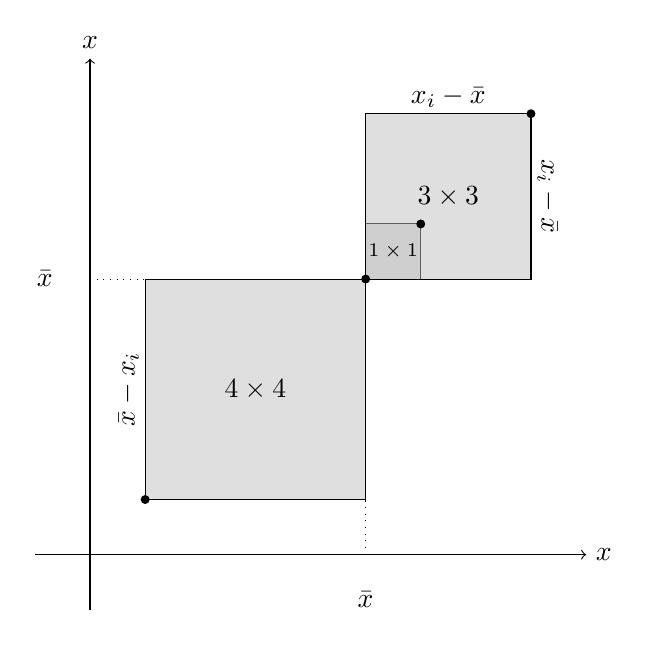
\begin{tikzpicture}[scale=.7]
    % Draw the squares and label their areas
    \foreach \x/\y in {1/1, 5/5, 6/6, 8/8}{
      \fill[gray!50,opacity=0.5] (\x,\y) rectangle ({5},{5});
      \draw (\x,\y) rectangle ({5},{5});
    }
      \node at (6.5,8.3) {$x_i - \bar{x}$};
    \node[rotate=-90] at (8.3,6.5) {$x_i - \bar{x}$};
    \node[rotate=90] at (.7,3) {$\bar{x}-x_i$};
    % Draw the rectangle at (5,5) and label its area
    % Draw the points
    \foreach \x/\y in {1/1, 5/5, 6/6, 8/8}{
      \filldraw[black] (\x,\y) circle (2pt);
    }
    % Draw the axes
    \draw[->] (-1,0) -- (9,0) node[right] {$x$};
    \draw[->] (0,-1) -- (0,9) node[above] {$x$};
    \draw[dotted] (5,0) -- (5,8);
    \node[below] at (5,-.5) {$\bar{x}$};
        \draw[dotted] (0,5) -- (8,5);
    \node[left] at (-.5, 5) {$\bar{x}$};
      \node at (3,3) {$4\times 4$};
        \node at (5.5,5.5) {\scriptsize{$1\times1$}};
          \node at (6.5,6.5) {$3\times 3$};
  \end{tikzpicture}
  \end{column}
  \begin{column}{0.5\textwidth}
 \begin{align*}
 \widehat{Var}(X)&=\frac{1}{N}\sum_i(x_i-\bar{x})(x_i-\bar{x})\\
 &=\frac{(-4*-4)+(1*1)+(3*3)}{4}\\
  &=\frac{26}{4}
 \end{align*} 
    \end{column}
  \end{columns}
\end{frame}


\begin{frame}
\begin{columns}
\begin{column}{0.5\textwidth}
  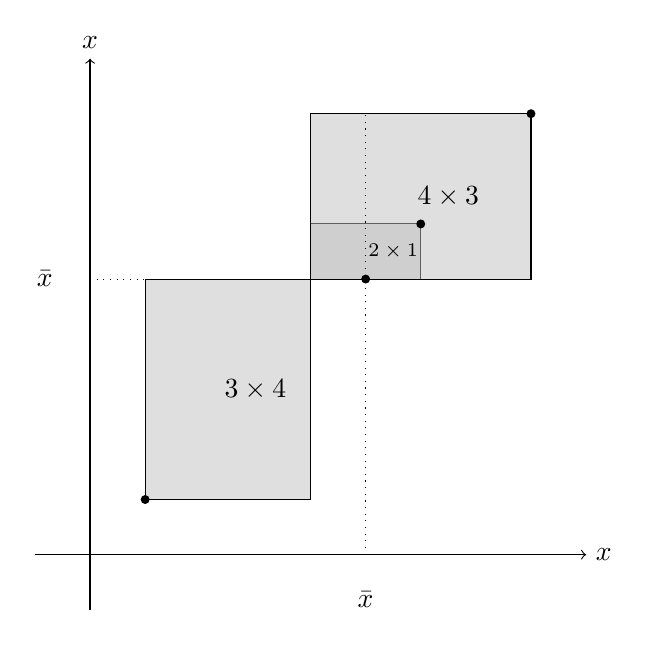
\begin{tikzpicture}[scale=.7]
    % Draw the squares and label their areas
    \foreach \x/\y in {1/1, 5/5, 6/6, 8/8}{
      \fill[gray!50,opacity=0.5] (\x,\y) rectangle ({4},{5});
      \draw (\x,\y) rectangle ({4},{5});
    }
    % Draw the rectangle at (5,5) and label its area
    % Draw the points
    \foreach \x/\y in {1/1, 5/5, 6/6, 8/8}{
      \filldraw[black] (\x,\y) circle (2pt);
    }
    % Draw the axes
    \draw[->] (-1,0) -- (9,0) node[right] {$x$};
    \draw[->] (0,-1) -- (0,9) node[above] {$x$};
    \draw[dotted] (5,0) -- (5,8);
    \node[below] at (5,-.5) {$\bar{x}$};
        \draw[dotted] (0,5) -- (8,5);
    \node[left] at (-.5, 5) {$\bar{x}$};
      \node at (3,3) {$3\times 4$};
        \node at (5.5,5.5) {\scriptsize{$2\times1$}};
          \node at (6.5,6.5) {$4\times 3$};
  \end{tikzpicture}
  \end{column}
  \begin{column}{0.5\textwidth}
   \begin{align*}
 \widehat{Var}(X)&=\frac{1}{N}\sum_i(x_i-\bar{x})(x_i-(\bar{x}-1))\\
 &=\frac{(-4*-3)+(1*2)+(3*4)}{4}\\
  &=\frac{26}{4}
 \end{align*} 
    \end{column}
  \end{columns}
\end{frame}


\begin{frame}
\begin{columns}
\begin{column}{0.5\textwidth}
  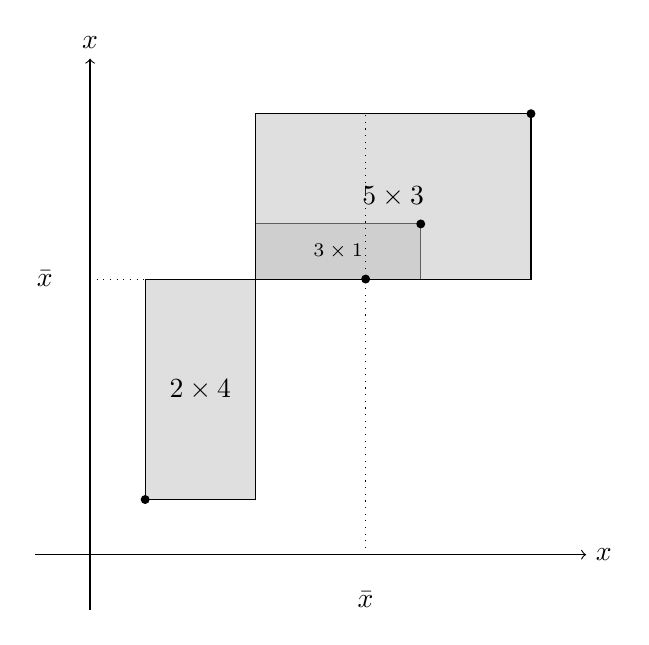
\begin{tikzpicture}[scale=.7]
    % Draw the squares and label their areas
    \foreach \x/\y in {1/1, 5/5, 6/6, 8/8}{
      \fill[gray!50,opacity=0.5] (\x,\y) rectangle ({3},{5});
      \draw (\x,\y) rectangle ({3},{5});
    }
    % Draw the rectangle at (5,5) and label its area
    % Draw the points
    \foreach \x/\y in {1/1, 5/5, 6/6, 8/8}{
      \filldraw[black] (\x,\y) circle (2pt);
    }
    % Draw the axes
    \draw[->] (-1,0) -- (9,0) node[right] {$x$};
    \draw[->] (0,-1) -- (0,9) node[above] {$x$};
    \draw[dotted] (5,0) -- (5,8);
    \node[below] at (5,-.5) {$\bar{x}$};
        \draw[dotted] (0,5) -- (8,5);
    \node[left] at (-.5, 5) {$\bar{x}$};
      \node at (2,3) {$2\times 4$};
        \node at (4.5,5.5) {\scriptsize{$3\times1$}};
          \node at (5.5,6.5) {$5\times 3$};
  \end{tikzpicture}
  \end{column}
  \begin{column}{0.5\textwidth}
   \begin{align*}
 \widehat{Var}(X)&=\frac{1}{N}\sum_i(x_i-\bar{x})(x_i-(\bar{x}-2))\\
 &=\frac{(-4*-2)+(1*3)+(3*5)}{4}\\
  &=\frac{26}{4}
 \end{align*} 

    \end{column}
  \end{columns}
\end{frame}


\begin{frame}
\begin{columns}
\begin{column}{0.5\textwidth}
  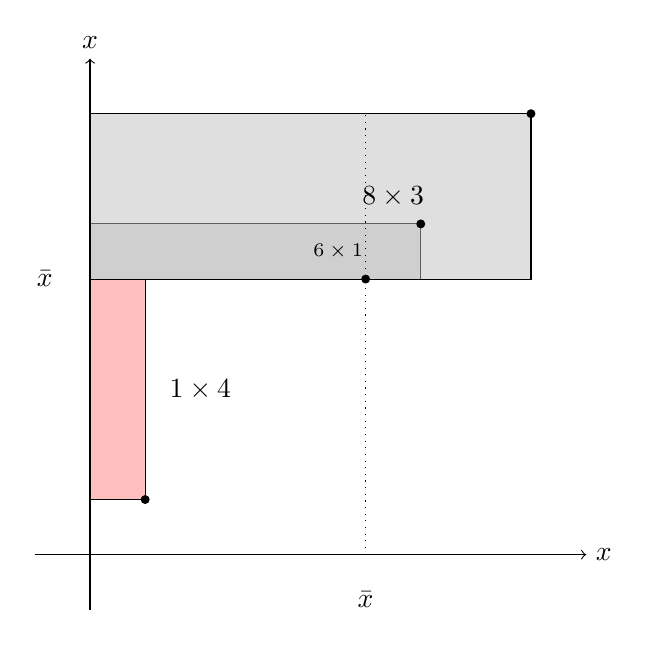
\begin{tikzpicture}[scale=.7]
    % Draw the squares and label their areas
    \foreach \x/\y in { 5/5, 6/6, 8/8}{
      \fill[gray!50,opacity=0.5] (\x,\y) rectangle ({0},{5});
      \draw (\x,\y) rectangle ({0},{5});
    }
    
      \fill[red!50,opacity=0.5] (1,1) rectangle ({0},{5});
      \draw (1,1) rectangle ({0},{5});
    
    % Draw the rectangle at (5,5) and label its area
    % Draw the points
    \foreach \x/\y in {1/1, 5/5, 6/6, 8/8}{
      \filldraw[black] (\x,\y) circle (2pt);
    }
    % Draw the axes
    \draw[->] (-1,0) -- (9,0) node[right] {$x$};
    \draw[->] (0,-1) -- (0,9) node[above] {$x$};
    \draw[dotted] (5,0) -- (5,8);
    \node[below] at (5,-.5) {$\bar{x}$};
        \draw[dotted] (0,5) -- (8,5);
    \node[left] at (-.5, 5) {$\bar{x}$};
      \node at (2,3) {$1\times 4$};
        \node at (4.5,5.5) {\scriptsize{$6\times1$}};
          \node at (5.5,6.5) {$8\times 3$};
  \end{tikzpicture}
  \end{column}
  \begin{column}{0.5\textwidth}
 \begin{align*}
 \widehat{Var}(X)&=\frac{1}{N}\sum_i(x_i-\bar{x})(x_i-(\bar{x}-\bar{x}))\\
 \widehat{Var}(X)&=\frac{1}{N}\sum_i(x_i-\bar{x})(x_i)\\
 &=\frac{(-4*1)+(1*6)+(3*8)}{4}\\
  &=\frac{26}{4}
 \end{align*} 

    \end{column}
  \end{columns}
\end{frame}



\begin{frame}
\frametitle{Example of Variance: Uniform} 

$X \sim \text{Uniform}(0,1)$.  What is $Var(X)$? \pause   

\begin{align*} 
E[X^2] & =  \int_0^1 X^2 \frac{1}{1-0}dx=\frac{X^3}{3}|_0^1\pause \\
 & =  \frac{1}{3}  \pause \\
E[X]^2 & =  \left(\frac{1}{2}\right)^2   
\end{align*}

\begin{align*}
Var(X) & = E[X^2] - E[X]^2  \pause  \\
& =  \frac{1}{3} - \frac{1}{4} = \alert{\frac{1}{12}}  
\end{align*}

\end{frame}


\section{Distributions}

\begin{frame}{Named Distributions: Normal}

\begin{defn}
Suppose $X$ is a random variable with $X \in \mathbf{R}$ and probability density function

\begin{align*}
f(x) & =  \frac{1}{\sqrt{2\sigma^2\pi}}\exp\left(-\frac{(x - \mu)^2}{2\sigma^2}\right) 
\end{align*}

Then $X$ is a \alert{normally} distributed random variable with parameters $\mu$ and $\sigma^2$.  \\

Equivalently, we'll write 
\begin{align*}
X & \sim  \text{Normal}(\mu, \sigma^2) 
\end{align*}

\end{defn}
\end{frame}




\begin{frame}{Discoverer of Normal Distribution}
\begin{center}
\includegraphics[width=1.8 in]{images/de_moivre.jpeg}\\
De Moivre (1711)
\end{center}
\end{frame}

\begin{frame}
\includegraphics[width=5.8 in]{images/NormalParameters.png}
\end{frame}



\begin{frame}{Named Distributions: $\chi^{2}$}

\begin{defn}
Suppose $X$ is a continuous random variable with $X\geq 0$, with PDF

\begin{align*}
f(x) &= g(n/2) x^{n/2 - 1} e^{-x/2} 
\end{align*}

Then we will say $X$ is a $\chi^2$ distribution with $n$ degrees of freedom.  Equivalently,

\begin{align*}
X & \sim  \chi^{2}(n) 
\end{align*}

\end{defn}
\begin{itemize}
\item $X = \sum_{i=1}^{N} Z^2$, where $Z\sim N(0,1)$
\end{itemize}

\end{frame}


\begin{frame}{Chi-Squares, p-values, histograms}
\begin{center}
\includegraphics[width=1.7 in]{images/Pearson.jpeg}\\
Pearson (1901)
\end{center}
\end{frame}


\begin{frame}
\frametitle{Student's $t$-Distribution}

\begin{defn}
Suppose $Z \sim \text{Normal}(0, 1)$ and $U \sim \chi^2(n)$.  Define the random variable $Y$ as, 

\begin{align*}
Y &= \frac{Z}{\sqrt{\frac{U}{n}}}
\end{align*}

If $Z$ and $U$ are independent then $Y \sim t(n)$, with PDF

\begin{align*}
f(x) &= h(n) \left(1 + \frac{x^2}{n}\right)^{-\frac{n+1}{2}} 
\end{align*}

We will use the t-distribution extensively for \alert{test-statistics}


\end{defn}

\end{frame}

%
%\begin{frame}
%\frametitle{Student's $t$-Distribution, Properties}
%\begin{columns}
%\begin{column}{0.5\textwidth}
%Suppose $n = 1$, \alert{Cauchy} distribution
%
%\scalebox{0.25}{\includegraphics{Cauchy1.png}} 
%\end{column}
%\begin{column}{0.5\textwidth}
%If $X \sim \text{Cauchy}(1)$, then:\\\pause
%$E[X] =$ undefined \\ \pause
%var$(X)$ = undefined \\ \pause
%
%If $X \sim t(2)$ \\ \pause
%E[X] = 0  \\\pause
%$\text{var}(X) $ = undefined
%\end{column}
%\end{columns}
%
%\end{frame}
%
%
%\begin{frame}
%\frametitle{Student's $t$-Distribution, Properties}
%
%Suppose $n>2$, then \\
%$var(X) = \frac{n}{n-2}$ \\
%As $n \rightarrow \infty$ var$(X) \rightarrow 1$.  
%
%
%
%\end{frame}
%


\begin{frame}
\frametitle{Using the t-Distribution}
Suppose we take $N$ iid draws, 
\begin{align*}
X & \sim  \text{Normal}(\mu, \sigma^2) 
\end{align*}

Define our data set $\boldsymbol{x} = (x_{1}, \hdots, x_{N})$

Calculate:
\begin{align*}
 \bar{x} & =   \sum_{i=1}^{N} \frac{x_{i}}{N} \\
 s^2 & =  \frac{1}{N-1} \sum_{i=1}^{N} (x_{i} - \bar{x})^2\\
t & =  \frac{\bar{x} - \mu}{s/\sqrt{N}}  \\
t & \sim Student's\ t(N-1) 
\end{align*}
\end{frame}

\begin{frame}{Example}
10 measurements from a normally distributed $x$ to test whether $\mu=80$.\\
Step 1: Calculate the sample mean, 
$$\bar{x}=\frac{83 + 93 + 147+ 102+ 104+ 151+ 114+ 62+79+ 87}{10}=102.2$$
Step 2: Calculate the sample standard deviation, 
$$s^2=\frac{(-19.2^2+ -9.2^2+ 44.8^2 -0.2^2 +1.8^2+ 48.8^2+ 11.8^2-40.2^2  -23.2^2 -15.2^2)}{9}=818.8$$
Step 3: Calculate test statistic, 
$$t=\frac{102.2-H_0}{\frac{\sqrt{818.8}}{\sqrt{10}}},\quad \frac{102.2-80}{\frac{\sqrt{818.8}}{\sqrt{10}}}=2.4533$$
Step 4: Calculate p-value,
$$2*(1-pt(2.4533,9))=.0365$$
\end{frame}



\section{Joint Dist.}



\begin{frame}{Joint PDFs}
If we want to know the probability of a set of joint events $(x, y) \in A$
$$P((X,Y)\in A)=\int_{y\in A}\int_{x\in A}  f_{X,Y}(x, y) dxdy$$\pause

We can also calculate the PDFs of X and Y individually (these are the marginal distributions):
$$f_X(x)=\int_y f_{X,Y}(x, y)dy, \ \ \quad f_Y(y)=\int_x f_{X,Y}(x, y)dx$$

\end{frame}






\begin{frame}
\frametitle{Example of Joint Probability Density: Roof}
$$f_{X,Y}(x,y) = x+y,\ \quad for\ x,\ y\ \in [0,1]$$\pause
the marginal densities $f_X(x)$ and $f_Y(y)$ are
$$f_X(x)=\int_0^1(x+y)dy= xy+\frac{y^2}{2}|_0^1= x+\frac{1}{2}$$\pause
$$f_Y(y)=\int_0^1(x+y)dx=\frac{x^2}{2}+yx|_0^1=\frac{1}{2}+y$$
\end{frame}



\begin{frame}{Example of Joint Probability Density: Quarter Circle}
\begin{align*}
f_{X,Y}(x,y) &= 3/2 \quad \text{ for }x^2\leq y\leq 1 \text{ and }0\leq x\leq 1\\\pause
\end{align*}

\begin{align*}
f_X(x) &= \int_{-\infty}^\infty f(x,y) dy =\int_{x^2}^1\frac{3}{2} dy\\
&=\frac{3}{2}y|_{x^2}^1=\frac{3}{2}(1-x^2)\\
f_Y(y) &= \int_{-\infty}^\infty f(x,y) dx=\int_{0}^{\sqrt{y}}\frac{3}{2} dx\\
&=\frac{3}{2}x|_{0}^{\sqrt{y}}=\frac{3}{2}\sqrt{y}
\end{align*}

\end{frame}


\begin{frame}{Plotting the Quarter Circle Distribution}

x $<$- seq(0, 1, 0.01)\\
y $<$- seq(0, 1, 0.01)\\
z $<$- outer(x, y, function(x, y)\{ ifelse(y$>x^2$, 2/3,0)\})\\
persp(x, y, z)

\end{frame}


\begin{frame}
\begin{center}
\includegraphics[width=3 in]{images/halfcircle.pdf}
\end{center}
\end{frame}


\begin{frame}{Plotting the Roof Distribution $f(x,y)=x+y$}

x $<$- seq(0, 1, 0.01)\\
y $<$- seq(0, 1, 0.01)\\
z $<$- outer(x, y, function(x, y)\{ x + y \})\\
persp(x, y, z)

\end{frame}


\begin{frame}
\begin{center}
\includegraphics[width=3 in]{images/roof.pdf}
\end{center}
\end{frame}

\section{Covariance}

\begin{frame}
\frametitle{Covariance} 

\begin{defn} 
For jointly continuous random variables $X$ and $Y$ define, the covariance of $X$ and $Y$ as,\pause 
\begin{align*}
\text{Cov}(X,Y) & =  E[(X-E[X])(Y- E[Y])]  \pause  \\
& =  E\left[ XY - E[X] Y - E[Y] X + E[X]E[Y] \right]  \pause  \\
& =  E[XY] - 2E[X]E[Y] + E[E[X]E[Y]]   \pause \\
& =  E[XY] - E[X]E[Y] \pause 
\end{align*}
\end{defn} 
Note, $E[XY]=\int_x\int_y xy f(x,\ y)dy dx$
\end{frame}


\begin{frame}{Correlation}
\begin{defn} 
Define the correlation of $X$ and $Y$ as,  \pause 
\begin{align*}
\text{Cor}(X,Y) & =  \frac{\text{Cov}(X,Y) }{\sqrt{\text{Var}(X) \text{Var}(Y) } }
\end{align*}
\end{defn} 
\end{frame}


\begin{frame}
\frametitle{Covariance facts}

Variance is the covariance of a random variable with itself.\pause 
\begin{align*}
Cov(X,X) & =  E[X X] - E[X]E[X] \pause \\
& =  E[X^2] - E[X]^2
\end{align*}
\pause 
Correlation measures the linear relationship between two random variables\\ 

\begin{align*}
E(XY) & =  \sigma_{XY}+\mu_X\mu_Y  \\
E(X^2) & =  \sigma^2_{X}+\mu^2_X  \\
\end{align*}

\end{frame}


\begin{frame}{Correlation$=.816$}
\includegraphics[width=3.5 in]{images/Anscomb.png}
\end{frame}


\begin{frame}{Correlation and Covariance}
Suppose $X = Y$ \pause 
\begin{align*}
Cor(X,Y) &= \frac{Cov(X,Y)}{\sqrt{Var(X)Var(Y)} }  \\ \pause 
&= \frac{Var(X)}{Var(X)}  \\ \pause 
&= 1   \pause 
\end{align*}

Suppose $X = -Y$  \pause 
\begin{align*}
Cor(X,Y) &= \frac{Cov(X,Y)}{\sqrt{Var(X)Var(Y)} } \\ \pause 
& =   \frac{- Var(X)}{Var(X)}  \\
& =   -1
\end{align*}

\end{frame}

\begin{frame}
\frametitle{Example covariance X, Y: $f(x,y)=X + Y$} 
Suppose $X$ and $Y$ have joint probability distribution $x + y$ for $x,\ y \in [0,1]$.  \pause \\
\begin{columns}
\begin{column}{0.5\textwidth}
\begin{align*}
E[XY] &= \int_{0}^{1} \int_{0}^{1} xy (x + y) dx dy \pause \\
&= \int_{0}^{1} \int_{0}^{1} (x^2 y + y^2 x) dx dy   \pause \\
&= \int_{0}^{1}(\frac{x^3 y}{3} + \frac{y^2 x^2}{2}|_0^1 )dy   \pause \\
&= \int_{0}^{1} (\frac{y}{3} + \frac{y^2}{2} ) dy  \pause \\
&= \frac{1}{6} + \frac{1}{6} = \frac{1}{3} \pause  
\end{align*}
\end{column}
\begin{column}{0.5\textwidth}
\begin{align*}
E[X] &= \int_{0}^{1} \int_{0}^{1} x (x + y) dxdy  \pause \\
 &= \int_{0}^{1}\frac{x^3}{3} + y\frac{x^2}{2}) |_0^1dy  \pause \\
 &= \int_{0}^{1}(\frac{1}{3} + \frac{y}{2})dy  \pause \\
  &= \frac{y}{3} + \frac{y^2}{4} |_0^1  \pause \\
   &= \frac{1}{3} + \frac{1}{4} = \frac{7}{12} 
 \end{align*}
 \end{column}
\end{columns}

\end{frame}




\begin{frame}
\frametitle{Example: $X + Y$ } 

\begin{align*}
\text{Cov}(X,Y) &=  E[XY] - E[X]E[Y]   \pause \\
&= \frac{1}{3}  - \frac{7}{12} *\frac{7}{12}   \pause \\
&= \frac{1}{3}  - \frac{49}{144} = -\frac{1}{144}   \pause 
\end{align*}

\begin{align*}
\text{Cor}(X,Y) &= \frac{\text{Cov}(X,Y)}{\sqrt{\text{Var}(X) \text{Var}(Y) }} \pause \\
&= \frac{- \frac{1}{144}}{\frac{11}{144}}  \pause  \\
&= \frac{-1}{11}  
\end{align*}


\end{frame}


\section{Conditional Prob.}

\begin{frame}
\frametitle{Conditional Probability Distribution Function}
\begin{defn}
Suppose $X$ and $Y$ are random variables with joint PDF $f(x,y)$.  Then define the \alert{conditional probability distribution} $f(x|y)$ as 

\begin{align*}
f(x|y) &= \frac{f(x, y) }{f_{Y}(y) } \\
f(x|y)f_{Y}(y)&= f(x, y)   
\end{align*}

\end{defn}

\end{frame}



\begin{frame}{Examples of Conditional Distributions (roof)}
\begin{itemize}
\item Roof Distribution:
\begin{align*}
f_{X,Y}(x,y)&=x+y\\
f_{X|Y}(x|y)&=\frac{f_{X,Y}(x,y)}{f_Y(y)}=\frac{x+y}{\frac{1}{2}+y}
\end{align*}
\item Quarter circle distribution:
\begin{align*}
f_{X,Y}(x,y)&=3/2 \quad \text{ for }y^2\leq x\leq 1 \text{ and }0<y<1\\
f_{X|Y}(x|y)&=\frac{f_{X,Y}(x,y)}{f_Y(y)}=\frac{3/2}{\frac{3}{2}\sqrt{y}}
\end{align*}
\end{itemize}


\end{frame}


\begin{frame}
\frametitle{Conditional Expectation}
$$\mathbb{E}(Y|X)=\int y\cdot f_{Y|X} (y|x)dy $$
$\mathbb{E}(Y|X)$ is the \emph{best} way to predict Y given X.

\end{frame}


\begin{frame}
\frametitle{Example of Conditional Expectation}
\begin{align*}
E(Y|X)&=\int_0^1 y f_{Y|X}(y|x)dy\\ \pause
&=\int_0^1 y \big(\frac{x+y}{\frac{1}{2}+x}\big)dy \\\pause
&=\frac{1}{x+\frac{1}{2}}\int_0^1 y (x+y)dy\\\pause
&=\frac{1}{x+\frac{1}{2}} \big(\frac{y^2x}{2} +\frac{y^3}{3}\big) |_0^1\\\pause
&=\frac{2+3x}{3+6x}
\end{align*}
\end{frame}


\begin{frame}
\begin{center}
\includegraphics[width=3in]{images/ConditionalExp1.pdf}
\end{center}
\end{frame}




\begin{frame}
\frametitle{Height (X) and Age (Z): Covariance}

We said the height of a child is distributed $f(x)=N(\mu=33+z*2, s= 1.2)$.  \\
Recall $f(x,z)=f(x|z)f(z)$ and that $f(x)=f(x|z=6).5+f(x|z=7).5$
\begin{align*}
Cov(x,z)&=E[xz]-E[x]E[z]  \quad \textit{ from definition}\\\pause
&=\sum\int xz f(x,z)dx- \int x f(x) \sum z f(z)\\\pause
&=(\int x*6 f(x|z=6)f(z=6)dx+\int x*7 f(x|z=7)f(z=7)dx)- 46*6.5\\\pause
&=(\int x*6 f(x|z=6).5dx+\int x*7 f(x|z=7).5dx)- 46*6.5\\\pause
&=3*\int x f(x|z=6)dx+3.5*\int x f(x|z=7)dx)- 46*6.5\\\pause
&=(3*45+3.5*47)- 46*6.5 =299.5-299\\\pause
&=0.5
\end{align*}
\end{frame}

\begin{frame}
\frametitle{Height (X) and Age (Z): Covariance}

Given  $$f(x)=N(\mu=33+z*2, s= 1.2)$$
$$Var(Z)=p*(1-p)=.25$$
Then $$\frac{Cov(x,z)}{var(z)}=.5/.25=2$$\pause

$$E(X|Z)=33+z*2$$

\end{frame}


\begin{frame}
\frametitle{Height (X) and Age (Z): Variances}
$$\sigma^2+E(X)^2=E(X^2)$$
Correlation requires Var(X):
\begin{align*}
f(x)&=.5*N(45,\ 1.2)+.5*N(47,\ 1.2)\ \ \quad \textit{ by assumption.}\\\pause
E(x)&=\sum p_i E[x_i] \ \quad \textit{ when we have a mixture of distributions with weights $p$}\\\pause
Var(x)&=\sum p_i E[x_i^2]-[\sum p_i E[x_i]]^2\\\pause
Var(x)&=.5*E(X_1^2)+.5*E(X_2^2)-(.5*E(X_1)+.5*E(X_1))^2\\\pause
Var(x)&=.5*(\sigma_1^2+E(X_1)^2)+.5*(\sigma_2^2+E(X_2)^2)-(.5*E(X_1)+.5*E(X_2))^2\\\pause
Var(x)&=.5*(1.2^2+45^2)+.5*(1.2^2+47^2)-(.5*45+.5*47)^2\\\pause
Var(x)&=2.44
\end{align*}
\end{frame}

\begin{frame}
\frametitle{Height (X) and Age (Z): Correlation}
The correlation:
\begin{align*}
Cor(x,z)&=\frac{Cov(x,z)}{\sqrt{Var(x)Var(z)}}\\
Cor(x,z)&=\frac{.5}{\sqrt{2.44*.25}}\\
Cor(x,z)&=0.64
\end{align*}

Note, we saw the regression coefficient: Cov(x,z)/Var(z)=2. \\
We will show that:
$$r_{x,z}*\frac{s_x}{s_z}=b_1$$
$$0.64*\frac{\sqrt{2.44}}{\sqrt{0.25}}=2$$
\end{frame}


\begin{frame}
\frametitle{Independence and Covariance}

\begin{prop}
Suppose $X$ and $Y$ are independent.  Then 
\begin{align*}
\text{Cov}(X, Y) &= 0  
\end{align*}

\end{prop}

\end{frame}


\begin{frame}
\frametitle{Independence and Covariance}
\begin{small}
\begin{proof}
Suppose $X$ and $Y$ are independent.  \pause 
\begin{align*}
\text{Cov}(X, Y) &= E[XY] - E[X]E[Y]   \pause 
\end{align*}

Calculating $E[XY]$ \pause 
\begin{align*}
E[XY] &= \int_{-\infty}^{\infty} \int_{-\infty}^{\infty} x y f(x,y)dxdy  \\ \pause 
& = \int_{-\infty}^{\infty} \int_{-\infty}^{\infty} x y f_{X}(x) f_{Y}(y)dxdy  \\ \pause 
&= \int_{-\infty}^{\infty} x f_{X}(x) dx \int_{-\infty}^{\infty} y f_{Y}(y) dy  \\ \pause 
&= E[X] E[Y]  
\end{align*}
\end{proof}

\end{small}
\end{frame}


\section{LIE}

\begin{frame}
\frametitle{Iterated Expectations (LIE)}

\begin{prop}
Suppose $X$ and $Y$ are random variables.  Then 

\begin{align*}
E[X] &= E[E[X|Y]]  
\end{align*}


\end{prop}


\begin{itemize}
\item[-] Inner Expectation is $E[X|Y] = \int_{-\infty}^{\infty} x f_{X|Y} (x|y) dx$.  
\item[-] Outer expectation is over $y$.  
\item[-] This is analogous to the law of total probability.
\end{itemize}


\end{frame}


\begin{frame}
\frametitle{Iterated Expectations}

\begin{proof}
\begin{align*}
E[E[X|Y]] &= \int_{-\infty}^{\infty}  \int_{-\infty}^{\infty} x f_{X|Y} (x|y) f_{Y}(y) dx dy  \\ \pause 
&=  \int_{-\infty}^{\infty}  \int_{-\infty}^{\infty} x f_{X|Y} (x|y) f_{Y}(y) dy dx  \\ \pause 
&= \int_{-\infty}^{\infty} x \int_{-\infty}^{\infty}  f(x, y) dy dx   \\ \pause 
&= \int_{-\infty}^{\infty}  x f_{X}(x) dx   \\ \pause 
&= E[X]  
\end{align*}
\end{proof}
\end{frame}


\begin{frame}
\frametitle{LIE Example: Proxy Fighting}
\begin{itemize}
\item  Suppose the US is seeking a local ally, but these come in three equally probable kinds, ``tough'', ``average'' and ``weak''.
\item The US would be willing to give \$11,000 per fighter if the group is strong, \$10,000 if the group is average, and \$0 if they are weak.\pause
\begin{itemize}
\item $E[price_{USA}]=E[E[price_{USA}|type]]=\sum_{type}E[price_{USA}|type]*p(type)$\pause
\item $E[price_{USA}]=\frac{1}{3}*(11k)+\frac{1}{3}*(10k)+\frac{1}{3}*(0)=7,000$\pause

\end{itemize}
\item The strong group will fight if they are paid \$10,000, the average group will fight if they are paid \$6,000, and the weak group would fight for \$50.\pause
\begin{itemize}
\item $E[price_{proxy}]=E[E[price_{proxy}|type]]=\sum_{type}E[price_{proxy}|type]*p(type)$\pause
\item $E[price_{proxy}]=\frac{1}{3}*(10k)+\frac{1}{3}*(6k)+\frac{1}{3}*(50)=5,350$\pause
\end{itemize}
\item If neither group knows their type, then they will be able to sell their services.
\end{itemize}
\end{frame}

\begin{frame}
\frametitle{LIE Example: Adverse Selection}
\begin{itemize}
\item  Suppose that the proxy knows their type but the US does not.\pause
\item If the US offers its average valuation of 7,000, it is only taken by the average and weak types.\pause
\item But, if tough proxies will not offer their services, the US would pay at most:
$$E[price_{USA}]=\frac{1}{2}10,000+\frac{1}{2}0=5,000$$
\item So even the average group will not fight.
\end{itemize}
\end{frame}

%
%\begin{frame}
%\frametitle{Next Steps}
%\begin{itemize}
%\item Read and work through "Estimators1", "Estimators2", "Estimators3.pdf"
%\item Finish working through "Proofsadvice.pdf"
%\end{itemize}
%\end{frame}
%
%\begin{frame}
%\frametitle{Law of Total Variance}
%Suppose $X$ and $Y$ are random variables.  Then 
%
%\begin{align*}
%var[X] &= E[var[X|Y]]+var(E[X|Y])  
%\end{align*}
%The first term is the average of the variation for each value of Y.\pause
%The second term is the variation across the averages within each value of Y.
%\end{frame}
%
%\section{Stats}
%
%\begin{frame}
%\frametitle{Estimators}
%\begin{itemize}
%\item We observe realizations from a vector of random variables $\boldsymbol{x}=(x_1, x_2 \ldots x_n)$. \pause
%\item When we construct a function $z(\boldsymbol{x})$ of observed data, they are called `statistics'. \pause  
%\item If that function is used to infer the value of a parameter of a distribution, it is called an `estimator'.\pause
%\item All estimators are random variables with distributions.\pause
%\begin{itemize}
%\item $\bar{x}(\boldsymbol{x})=\frac{\sum x_i }{n}$ is the sample mean and estimates the true mean ($\mu$). \pause
%\item $s^2(\boldsymbol{x})=\frac{\sum (x_i-\bar{x})^2 }{n-1}$ is the sample variance and estimates  the true variance ($\sigma^2$).\\ \pause
%\end{itemize}
%\item An estimator $\hat{\theta}$ is evaluated by its expectation and variance.
%\begin{itemize}
%\item Is $E(\hat{\theta})-\theta=0$?  If so, it is called unbiased.
%\item Is $var(\hat{\theta})\leq var(\tilde{\theta})$, where $\tilde{\theta}$ is any other unbiased estimator?  If so, it is called efficient.
%\item How does $\hat{\theta}_n$ behave as $n$ gets arbitrarily large? Next time. 
%\end{itemize}
%\end{itemize}
%\end{frame}
%
%\begin{frame}
%\frametitle{Preview: Sample Mean is unbiased}
%\begin{itemize}
%\item If $\boldsymbol{x}=(x_1, x_2 \ldots x_n)$ are a iid random sample drawn from some distribution with mean $\mu$, and we calculate $\bar{x}(\boldsymbol{x})=\frac{1}{N}\sum_{i=1}^N x_i$, we can show that $E[\bar{x}]-\mu=0$:
%\begin{align*}
%E[\bar{x}(\boldsymbol{x})]&=E[\frac{1}{N}\sum_{i=1}^N x_i]\\
%&=\frac{1}{N}[\sum_{i=1}^N E[x_i]]\\
%&=\frac{1}{N}[\sum_{i=1}^N \mu]\\
%&=\frac{1}{N}[N \mu]\\
%&=\mu
%\end{align*}
%\end{itemize}
%\end{frame}


\end{document}
